\documentclass[a4paper, man, floatsintext]{apa6}
\usepackage{lmodern}
\usepackage{amssymb,amsmath}
\usepackage{ifxetex,ifluatex}
\usepackage{fixltx2e} % provides \textsubscript
\ifnum 0\ifxetex 1\fi\ifluatex 1\fi=0 % if pdftex
  \usepackage[T1]{fontenc}
  \usepackage[utf8]{inputenc}
\else % if luatex or xelatex
  \ifxetex
    \usepackage{mathspec}
  \else
    \usepackage{fontspec}
  \fi
  \defaultfontfeatures{Ligatures=TeX,Scale=MatchLowercase}
\fi
% use upquote if available, for straight quotes in verbatim environments
\IfFileExists{upquote.sty}{\usepackage{upquote}}{}
% use microtype if available
\IfFileExists{microtype.sty}{%
\usepackage{microtype}
\UseMicrotypeSet[protrusion]{basicmath} % disable protrusion for tt fonts
}{}
\usepackage{hyperref}
\hypersetup{unicode=true,
            pdfauthor={Jana B. Jarecki},
            pdfborder={0 0 0},
            breaklinks=true}
\urlstyle{same}  % don't use monospace font for urls
\usepackage{graphicx,grffile}
\makeatletter
\def\maxwidth{\ifdim\Gin@nat@width>\linewidth\linewidth\else\Gin@nat@width\fi}
\def\maxheight{\ifdim\Gin@nat@height>\textheight\textheight\else\Gin@nat@height\fi}
\makeatother
% Scale images if necessary, so that they will not overflow the page
% margins by default, and it is still possible to overwrite the defaults
% using explicit options in \includegraphics[width, height, ...]{}
\setkeys{Gin}{width=\maxwidth,height=\maxheight,keepaspectratio}
\IfFileExists{parskip.sty}{%
\usepackage{parskip}
}{% else
\setlength{\parindent}{0pt}
\setlength{\parskip}{6pt plus 2pt minus 1pt}
}
\setlength{\emergencystretch}{3em}  % prevent overfull lines
\providecommand{\tightlist}{%
  \setlength{\itemsep}{0pt}\setlength{\parskip}{0pt}}
\setcounter{secnumdepth}{0}
% Redefines (sub)paragraphs to behave more like sections
\ifx\paragraph\undefined\else
\let\oldparagraph\paragraph
\renewcommand{\paragraph}[1]{\oldparagraph{#1}\mbox{}}
\fi
\ifx\subparagraph\undefined\else
\let\oldsubparagraph\subparagraph
\renewcommand{\subparagraph}[1]{\oldsubparagraph{#1}\mbox{}}
\fi

%%% Use protect on footnotes to avoid problems with footnotes in titles
\let\rmarkdownfootnote\footnote%
\def\footnote{\protect\rmarkdownfootnote}

%%% Change title format to be more compact
\usepackage{titling}

% Create subtitle command for use in maketitle
\providecommand{\subtitle}[1]{
  \posttitle{
    \begin{center}\large#1\end{center}
    }
}

\setlength{\droptitle}{-2em}

  \title{}
    \pretitle{\vspace{\droptitle}}
  \posttitle{}
    \author{Jana B. Jarecki}
    \preauthor{\centering\large\emph}
  \postauthor{\par}
      \predate{\centering\large\emph}
  \postdate{\par}
    \date{20 November, 2019}

\usepackage{natbib} \usepackage{threeparttable} \usepackage{booktabs}
\shorttitle{test} \usepackage{setspace}
\AtBeginEnvironment{tabular}{\singlespacing} \usepackage{times}
\usepackage{changes} \definechangesauthor[name={JJ}, color=orange]{jj}
\usepackage{upgreek} \AtBeginDocument{\let\maketitle\relax}

\begin{document}

\subsubsection{Evaluations of gambles and sample sizes}

Analysis of the mean evaluations by sample size gives a similar picture
in Study\textasciitilde{}2 and Study\textasciitilde{}1 (Table
\ref{tab:means_study1}). Larger sample sizes did not lead to systematic
changes in evaluations of gambles (ANOVA with the predictors gamble type
and gamble expected value outperformed one with the added predictors
sample size (\(BF_{01}= 385\)) and a sample-size/gamble-type interaction
(\(BF_{02} > 1000\); models with by-participant random effects).
Replicating Study\textasciitilde{}1, there was a higher value assigned
to \$-bet gambles (\(M=4.69, SD=3.10\)) compared to the p-bet gambles
(\(M=5.25, SD=4.94\)), \(BF 0.69\) in favor of an ANOVA with criterion
evaluations and predictor gamble type over an ANOVA without the
predictor gamble type (both models include by-participant and
by-expected-value random effects). These results corroborate the
aggregate findings of Study 1.

\begin{table}[tbp]

\begin{center}
\begin{threeparttable}

\caption{\label{tab:means_study1}Valuations of Gambles in Study 1}

\begin{tabular}{lccccrr}
\toprule
Condition & Sample size category & Sample size & \textit{Med} & \textit{M} & D--E & D--E:$BF\textsubscript{10}$\\
\midrule
Gamble ID 1 (\$-bet) &  &  &  &  &  & \\
\ \ \ E & xs & 5 & 5.15 & 6.29 & -0.85 & 10\\
\ \ \ E & s & 10 & 5.00 & 6.39 & -0.96 & 354\\
\ \ \ E & m & 15 & 5.95 & 6.38 & -0.95 & 71\\
\ \ \ E & l & 30 & 6.00 & 6.53 & -1.09 & 163\\
\ \ \ D & -- & -- & 4.00 & 5.43 & -- & --\\
Gamble ID 2 (\$-bet) &  &  &  &  &  & \\
\ \ \ E & xs & 6 & 4.00 & 4.55 & -0.24 & 0\\
\ \ \ E & s & 12 & 4.00 & 4.72 & -0.41 & 1\\
\ \ \ E & m & 18 & 5.00 & 4.88 & -0.57 & 4\\
\ \ \ E & l & 36 & 4.95 & 4.78 & -0.47 & 4\\
\ \ \ D & -- & -- & 3.35 & 4.31 & -- & --\\
Gamble ID 3 (\$-bet) &  &  &  &  &  & \\
\ \ \ E & xs & 7 & 8.95 & 10.65 & -1.41 & 6\\
\ \ \ E & s & 14 & 10.00 & 10.26 & -1.01 & 1\\
\ \ \ E & m & 21 & 9.70 & 10.37 & -1.12 & 2\\
\ \ \ E & l & 42 & 10.00 & 11.18 & -1.93 & 220\\
\ \ \ D & -- & -- & 6.00 & 9.25 & -- & --\\
Gamble ID 4 (p-bet) &  &  &  &  &  & \\
\ \ \ E & xs & 5 & 3.30 & 2.91 & 0.29 & 14\\
\ \ \ E & s & 10 & 3.20 & 2.94 & 0.26 & 25\\
\ \ \ E & m & 15 & 3.20 & 3.02 & 0.19 & 2\\
\ \ \ E & l & 30 & 3.20 & 3.09 & 0.11 & 0\\
\ \ \ D & -- & -- & 3.50 & 3.20 & -- & --\\
Gamble ID 5 (p-bet) &  &  &  &  &  & \\
\ \ \ E & xs & 6 & 2.00 & 1.82 & 0.10 & 1\\
\ \ \ E & s & 12 & 2.00 & 1.85 & 0.07 & 0\\
\ \ \ E & m & 18 & 2.00 & 1.85 & 0.06 & 0\\
\ \ \ E & l & 36 & 2.10 & 1.95 & -0.03 & 0\\
\ \ \ D & -- & -- & 2.00 & 1.92 & -- & --\\
Gamble ID 6 (p-bet) &  &  &  &  &  & \\
\ \ \ E & xs & 7 & 4.00 & 3.68 & 0.16 & 1\\
\ \ \ E & s & 14 & 4.10 & 3.78 & 0.07 & 0\\
\ \ \ E & m & 21 & 4.15 & 3.85 & -0.01 & 0\\
\ \ \ E & l & 42 & 4.20 & 3.90 & -0.05 & 0\\
\ \ \ D & -- & -- & 4.10 & 3.84 & -- & --\\
\bottomrule
\addlinespace
\end{tabular}

\begin{tablenotes}[para]
\normalsize{\textit{Note.} \textit{M} = mean, \textit{Med} = median, D--E = difference between mean description-based valuations and experience-based valuations, $BF\textsubscript{10}$ = Bayes Factor quantifying the evidence for a linear model $\mathrm{M}\textsubscript{1}$ predicting that valuations differ between description and experience over a linear model $\mathrm{M}\textsubscript{0}$ predicting no such differences; both models models contain a by-participant random effect. Gambles IDs 1, 2, and 3 are \$-bets; Gamble IDs 4, 5, and 6 are p-bets.}
\end{tablenotes}

\end{threeparttable}
\end{center}

\end{table}

\subsubsection{Cognitive modeling}

The modeling procedure followed Study 1.

\textit{Quantitative Model Fit.} More than half of the participants were
best-described by the Bayesian value updating model Bayesian value
updating model described the majority of the participants best (23 of
40; 57\%). The relative frequency model described 17 participants best
(42\%). The evidence strength of the models is shown in Figure
\ref{fig:fig2}. The models' mean Bayesian information criterion across
all participants equaled BIC\textsubscript{BVU}\(= -96\),
BIC\textsubscript{RF}\(= -91\), and BIC\textsubscript{BASE}\(= -17\)
(lower values indicate better fit).

\begin{figure}[htb]

{\centering 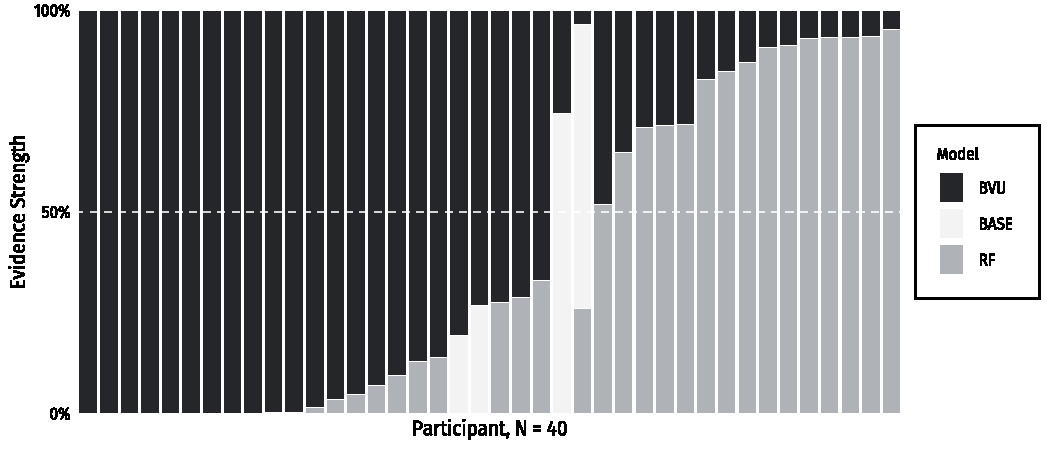
\includegraphics[width=.9\linewidth]{../figures/fig2-1} 

}

\caption{Evidence for the models for individual participants. \textit{RF}$=$ relative frequency model, \textit{BVU}$=$ Bayesian value updating model, \textit{BASE}$=$ Baseline model.}\label{fig:fig2}
\end{figure}

\added[id=jj]{
The fitted model parameters (\ref{tab:study1_parameter}) reveal that the power utility exponent did not differ markedly between the participants that were described by the Bayesian value updating strategy ($M_{\alpha}= 2.19$) and those described by a relative frequency strategy ($M_{\alpha}=2.15$), $\Delta$ $M = 0.02$ 95\% HDI $[-1.12$, $1.18]$, $\mathrm{BF}_{\textrm{01}} = 3.21$. Participants using the Bayesian strategy had, on average, a prior belief that gains occur with 45\% (gain prior $\theta_G = 0.91$; zero-outcome prior $\theta_0 = 1.09$). Also, their estimated learning rate $\delta$ was anti-conservative ($M_{\delta}=2.27$).
}

\begin{verbatim}
Error in `[.data.table`(tab, c(2, 3, 1), c("winner_n", "rp", "delta", : column(s) not found: m
\end{verbatim}

\textit{Qualitative Model Fit.} Figure \ref{fig:fig5} plots the
qualitative model fit (best-fitting model predictions against observed
evaluations by participant). As in Study 1, the data are generally
well-described
\added[id=jj]{($M r\textsubscript{pred,obs} = 0.70$), except in four cases (participants s42, s47, s54, s67, with $r\textsubscript{pred,obs} < 0.40$)}
where the model must be rejected because of qualitative mis-fit.

\begin{figure}[htb]

{\centering 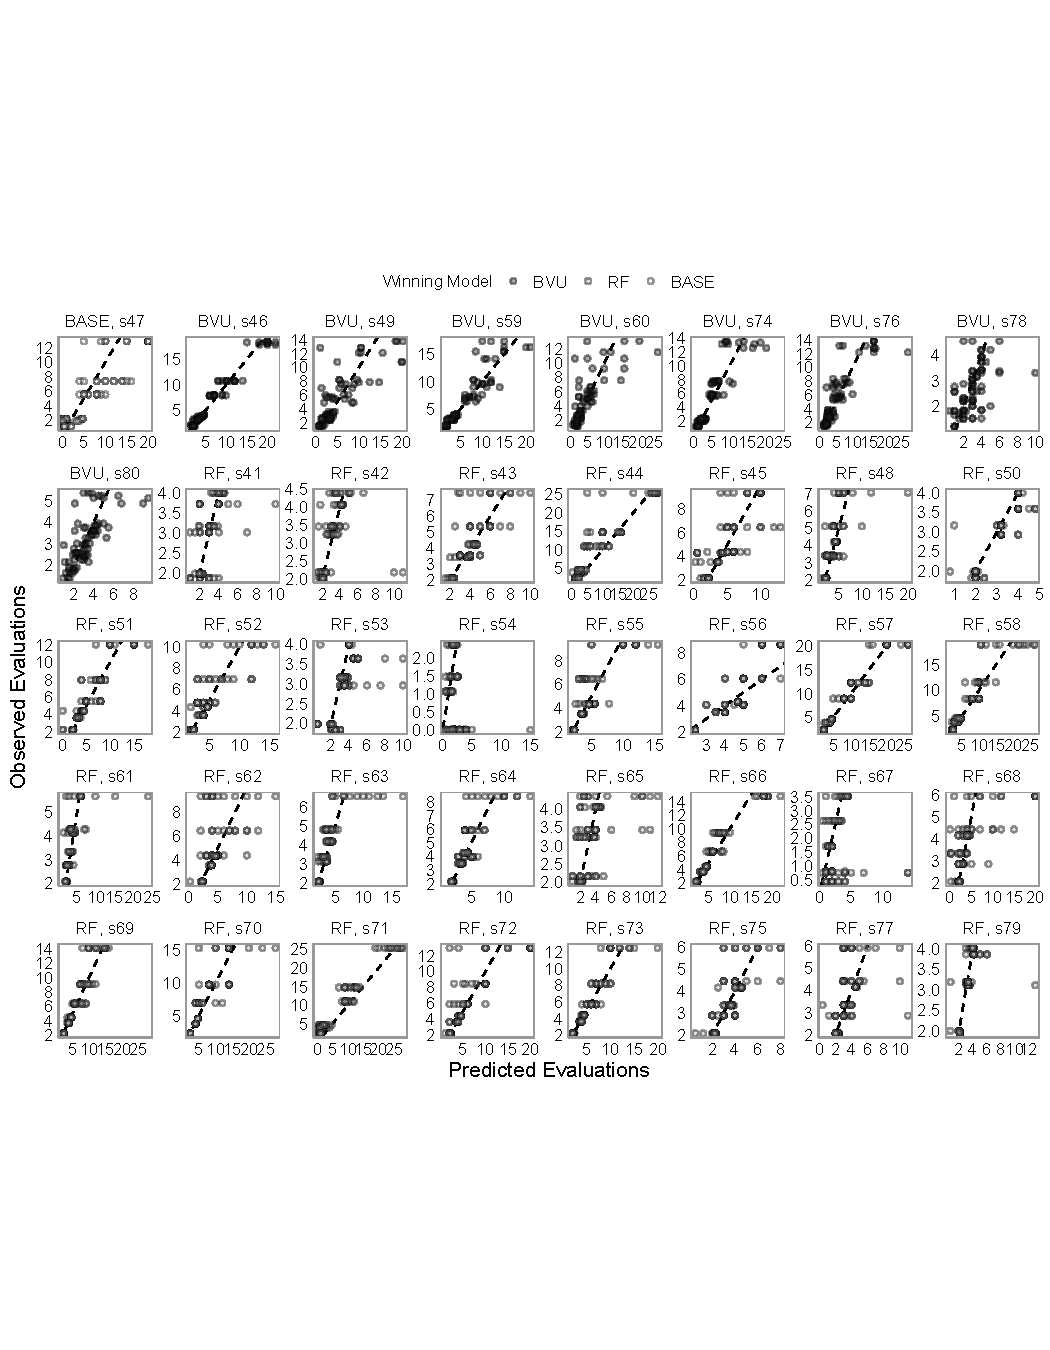
\includegraphics[width=\textwidth]{../figures/fig5-1} 

}

\caption{Predicted evaluations from the best-fitting models plotted against the observed evaluations (by participant). \textit{BVU}$=$ Bayesian value updating model, \textit{RF}$=$ relative frequency model, \textit{BASE}$=$baseline model.}\label{fig:fig5}
\end{figure}

\emph{The effect of sample size given cognitive strategies.} Next, we
qualitatively analyzed if sample size differentially affects the
relative-frequency-type and Bayesian-type learners. We expected that
sample size leads to changes in the evaluations of the Bayesian learners
depending on their priors, and that sample size does not affect the
evaluations of the relative-frequency learners.

\added[id=jj]{
The Bayesian model predicts that the evaluations are influenced by both sample size and prior beliefs. Participants with a gain prior---initially believing that gains are more likely than zero-outcomes---should decrease the evaluations of \$-bets as sample sizes increase, because participants learn that gains of \$-bets are less likely than zero-outcomes. By contrast, participants with a zero-outcome prior---initially believing that zero-outcomes are more likely than gains---should increase their evaluations of p-bets as sample size increases, because they learn that gains of p-bets are more likely than zero-outcomes.
}

\added[id=jj] {
  The cognitive modeling results show slightly greater strategy heterogeneity in Study 2 compared to Study 1 with a higher prevalence of the relative frequency strategy in Study 2. The higher prevalence of the relative frequency strategy in Study 2 can be explained by that the relative frequency strategy can be considered a cognitively simpler strategy and the fact that in Study 2 the outcomes were withheld from participants made learning in this design more demanding.
}

\added[id=jj]{Regarding confidence, the Bayesian model predict that the uncertainty about learners beliefs increases with more evidence, thus confidence should increase with sample size for Bayesian learners. The relative frequency model makes no predictions about confidence. In our data, however, the confidence of the $n = `winners["bvu"]`$ participants, who were best-described by the Bayesian value updating model, was unaffected by sample sizes with a low participant-level sample-size-confidence correlation ($M=0.04, SD=0.18$). A linear model\footnote{with by-participant random intercept and the predictors effect-coded.} of the confidence ratings, which excluded sample size as predictor, was preferred over a model including sample size ($BF\textsubscript{excl,incl} = < 1/1000$). Similarly, the confidence of the participants that were best described by the relative-frequency model was unaffected by sample size ($M = 4.20, 4.11, 4.14, 4.21$ for sample sizes s, xs, m, l, respectively; BF\textsubscript{excl,incl}$= 0$)}.

\textit{Description versus experience} The above Table
\ref{tab:means_study1} shows the mean and median valuations from
description and the difference between the mean valuations in the
experience and description conditions. Further, it provides the Bayes
factors, quantifying the evidence in favor of a difference between
valuations from experience and those from description.

Valuations made from description and experience differed for most of the
gambles and sample sizes (see Table \ref{tab:means_study1}, rightmost
column). In particular, participants attached a higher value to
experienced than to described \$-bets (Gambles 1--3) but attached a
higher value to described than to experienced p-bets (Gambles 4--6).
Thus, we found a D--E gap that is the opposite of the classic D--E gap
observed in choice paradigms. In our study, participants valued gambles
as if they overweighted rare events from description \textit{and}
experience. This effect was even stronger when people made valuations
from experience.


\end{document}
